\section*{Second Design}
The second design considered is a simple improvement over the first design which includes rounding before truncation a the output in an effort to improve resolution. This implementation will require another adder, though only eight bit instead of sixteen, that will increase the critical delay path from one multiplier and one adder to two adders and one multiplier. It should also be noted that this critical path will exist twice, refer to Figure \ref{subfig:block2-a}. This increase in overall delay and probability of use is reflected in the timing analysis. Unfortunately, the output waveform shows little improvement in terms of attenuation; see Figure \ref{subfig:output2-b}.  

\subsection*{Rounding Truncation}
The code used in the second design is uses an XOR gate to compare the ninth bit with the most significant or \"sign\" bit. In the case that the number is a negative two's complement number, if the ninth bit is zero, the output is rounded up by one (add one), otherwise, the least significant eight bits are simply truncated as with the first design. This process is inverter in the case of positive numbers.  \\*
\\*
xor xor1(s3, d3[15], d3[7]);\\*
add8 add3(d3[15:8], {7'b0, s3}, 1'b0, ad3, cout3);\\*
always @ (posedge clk)
begin\\*
y = ad3;\\*
end\\*
\\*
\subsection*{Second Design Timing Analysis}

% Table generated by Excel2LaTeX from sheet 'Sheet1'
\begin{table}[bh]
\caption{Xilinx Timing Report}
\begin{tabular}{c|c}
\centering
           & Timing in (ns) \\
\hline
Minimum Period &     \\

     Slack &     \\

Requrement &        \\

Data Path Delay &     \\
\end{tabular}  
\label{tab:timing2}
\end{table}

According to Table \ref{tab:timing2}, the maximum clock frequency for the second design has been calculated to be approximately:  MHz


\begin{figure}[htp]
  \begin{center}
    \subfigure[Functional block diagram]{\label{subfig:block2-a}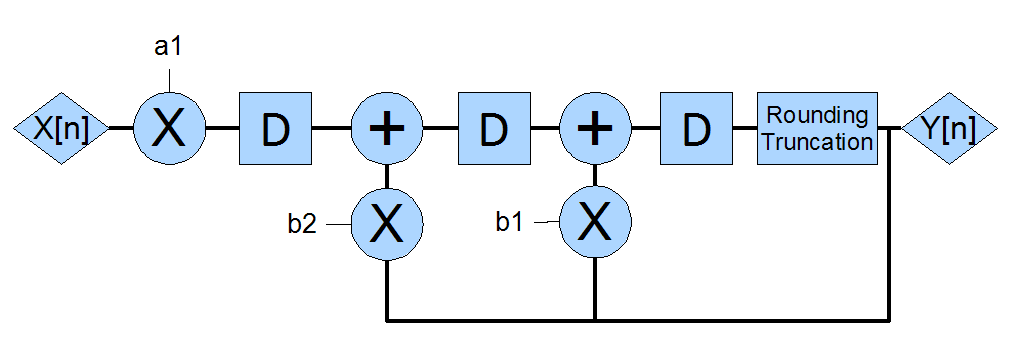
\includegraphics[scale=0.30]{block_two.png}}
    \subfigure[Input/Output comparison]{\label{subfig:output2-b}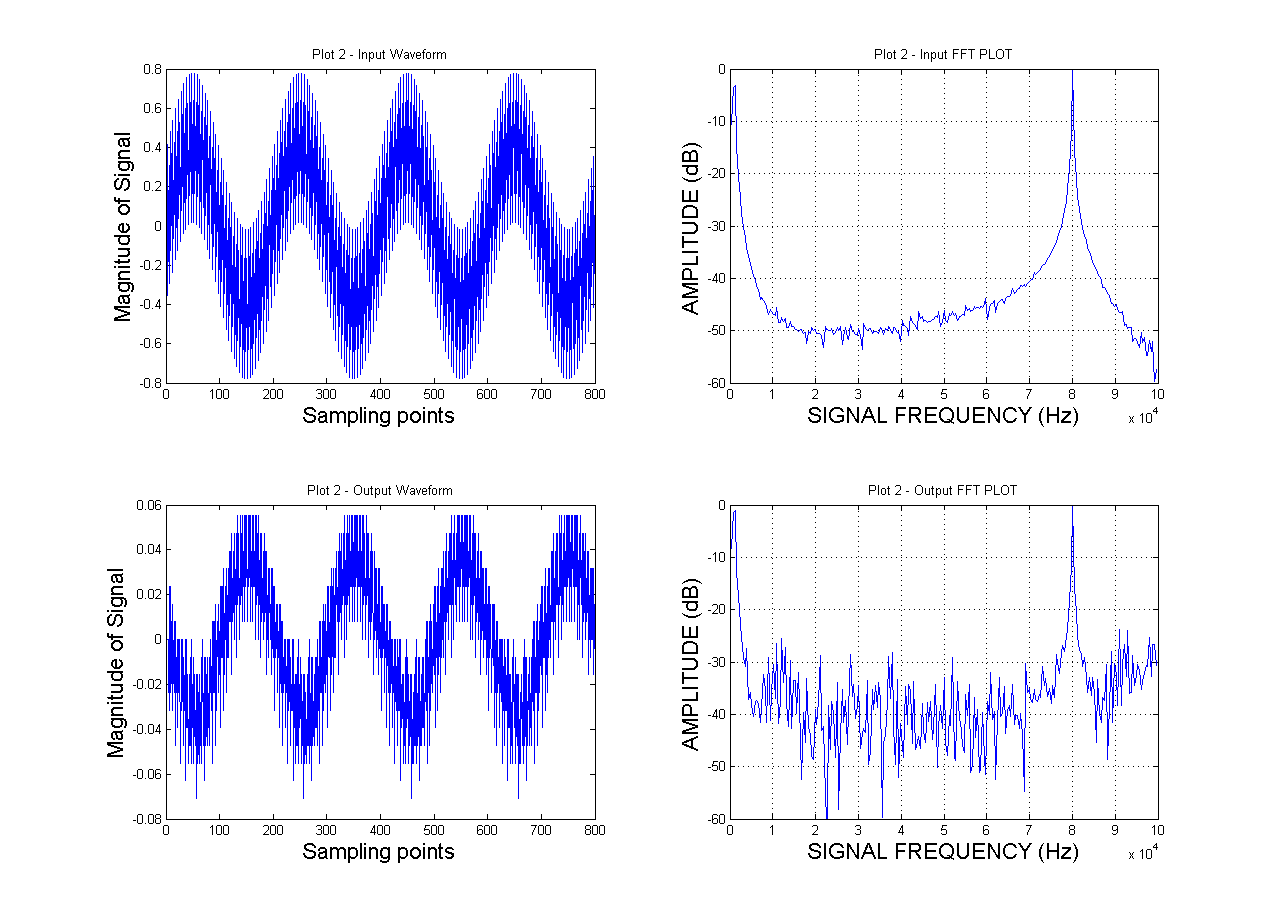
\includegraphics[scale=0.30]{plot2.png}} \\*
  \end{center}
  \caption{Second Design Results}
  \label{fig:design2_results}
\end{figure}